% ltex: language=it
\chapter{Classificazione}\label{chap:classificazione} % (fold)
\paragraph{Approccio Bayesiano}\label{par:approccio_bayesiano} % (fold)
Il problema è posto in  termini probabilistici.
\\
Se tutte le distribuzioni in gioco sono note l'approccio Bayesiano costituisce la migliore regola di classificazione possibile: soluzione \textbf{ottima}.
\\
\\
Sia $V$ uno spazio di pattern $d$-dimensionali e $W = \pg{w_1, w_2, \dots, w_s}$ un insieme di $s$ classi disgiunte costituite da elementi di $V$.
\\\\
Per ogni $x \in V$ e per ogni $\wi \in W$, indichiamo con $p\pt{x|\wi}$ la densità di probabilità condizionale (o condizionata) di $x$ data $\wi$, ovvero la densità di probabilità che il prossimo pattern sia $x$ sotto l'ipotesi che la sua classe di appartenenza sia $\wi$.
\\\\
Per ogni $\wi \in W$, indichiamo con $P\pt\wi$ la \textbf{probabilità a priori} di $\wi$, ovvero la probabilità, indipendentemente dall'osservazione, che il prossimo pattern da classificare sia di classe $\wi$.
\\\\
Per ogni $x \in V$ indichiamo con $p\pt x$ la densità di probabilità assoluta di $x$, ovvero la densità di probabilità che il prossimo pattern da classificare sia $x$:
\[
    p\pt x = \sum_{i = 1}^{s}{p\pt{x|\wi} \cdot P\pt\wi} \qquad\qquad\qquad \text{dove }\ \sum_{i = 1}^{s}{P\pt\wi} = 1
\]
\\
Per ogni $\wi \in W$ e per ogni $x \in V$ indichiamo con $P\pt{\wi|x}$ la \textbf{probabilità a posteriori} di $\wi$ dato $x$, ovvero la probabilità che avendo osservato il pattern $x$, la classe di appartenenza sia $\wi$.
Per il \textbf{teorema di Bayes}:
\begin{equation}\label{eq:theor-bayes}
    \ba{\wi}{x} = \dfrac{p\pt{x|\wi} \cdot \p\wi}{p\pt x}
\end{equation}
% paragraph Approccio Bayesiano (end)
%
\section{Classificatore di Bayes}\label{sub:classificatore_di_bayes} % (fold)
Dato un pattern $x$ da classificare in una delle $s$ classi $\wli, \wlii, \dots, w_s$ di cui sono note:
\begin{itemize}
    \item le \textbf{probabilità a priori}, $\p\wli, \p\wlii, \dots, \p{w_s}$;
    \item le \textbf{densità di probabilità condizionali}, $\dba{x}{\wli}, \dba{x}{\wlii}, \dots, \dba{x}{w_s}$;
\end{itemize}
la regola di classificazione di Bayes assegna $x$ alla classe $b$ per cui è massima la probabilità a posteriori:
\[
    b = \argmax_{i = 1, \dots, s}{\pg{\ba{\wi}{x}}}
\]
\begin{note}
    Massimizzare la probabilità a posteriori significa \textbf{massimizzare} la densità di probabilità condizionale tenendo comunque conto della probabilità a priori delle classi.
\end{note}
La regola si dimostra \textit{ottima} in quanto minimizza l'\textbf{errore di classificazione}.
Ad esempio nel caso di $2$ classi e $d = 1$:
\[
    \p{\text{error}} = \int_{\Re_1}{\dba{x}{w_2}\p\wlii\id} + \int_{\Re_2}{\dba{x}{w_1}\p\wli\,\id}
\]
\begin{cimage}
    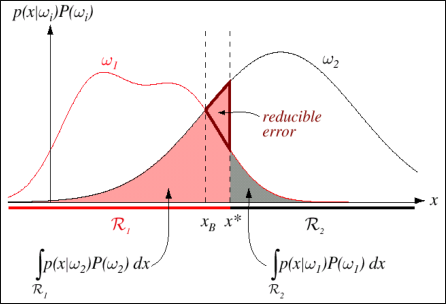
\includegraphics[width=.6\textwidth]{assets/bayes-class-graph.png}
    \caption{Rappresentazione dell'errore di classificazione}\label{fig:bayes-class-graph}
\end{cimage}
\begin{example}{Classificare maschi/femmine in base a peso e altezza}{maschi-femmine-bayes}
    \begin{center}
        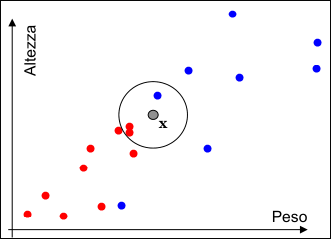
\includegraphics[width=.4\textwidth]{assets/training-set-es.png}
        \captionof{figure}{Training set di esempio}\label{fig:training-set-es}
    \end{center}
    A partire dal training set in \cref{fig:training-set-es}:
    \begin{itemize}
        \item $V$ è uno spazio a $2$ dimensioni, $d = 2$;
        \item $W = \pg{\wli, \wlii}$, dove $\wli$ sono i maschi (blu) e $\wlii$ sono le femmine (rosso)
    \end{itemize}
    Una stima (grossolana) delle probabilità a priori e delle densità può essere effettuata a partire dal training set come segue:
    \begin{itemize}
        \item \textbf{probabilità a priori} --- si considera semplicemente l'occorrenza dei pattern nel training set, in questo caso: $\p\wli = 8/18$, $\p\wlii = 10/18$;
        \item \textbf{densità di probabilità condizionali} --- per un nuovo pattern $x$ da classificare: si contano le occorrenze dei pattern nel training set delle due classi in un intorno di $x$:
            \begin{itemize}
                \item $\dba{x}{\wli} = 1/8$;
                \item $\dba{x}{\wlii} = 2/10 = 1/5$;
                \item $\dpb{x} = \frac{1}{8} \times \frac{8}{18} + \frac{1}{5} \times \frac{10}{18} = \frac{1}{18} + \frac{2}{18} = \frac{1}{6}$;
            \end{itemize}
    \end{itemize}
    Si ottiene quindi:
    \[
        \begin{matrix}
            \ba{\wli}{x} = \dfrac{\dba{x}{\wli} \cdot \p\wli}{\dpb x} = \dfrac{1/18}{1/6} = \dfrac{1}{3} \\\\
            \ba{\wlii}{x} = \dfrac{\dba{x}{\wlii} \cdot \p\wlii}{\dpb x} = \dfrac{2/18}{1/6} = \mathbf{\dfrac{2}{3}} \\\\
        \end{matrix}
    \]
    L'approccio Bayesiano assegna il pattern $x$ alla classe $w_2$ (femmine).
\end{example}
Mentre la stima delle probabilità a priori è abbastanza semplice, se non si hanno elementi si possono ipotizzare le classi equiprobabili, la \textbf{conoscenza} delle densità condizionali è possibile ``solo in teoria''; nella pratica esistono due soluzioni:
\begin{itemize}
    \item \textbf{Approccio parametrico};
    \item \textbf{Approccio non parametrico};
\end{itemize}
%
\subsection{Approccio parametrico}\label{sec:approccio_parametrico} % (fold)
Si fanno ipotesi sulla forma delle distribuzioni, es. \textit{distribuzione multinormale}, e si apprendono i parametri fondamentali (vettore medio, matrice di covarianza) dal training set.
\\
Generalmente utilizzato quando, oltre ad avere una ragionevole certezza (o \textit{speranza}) che la forma della distribuzione sia adeguata, la dimensione del training set non è sufficiente per una buona stima delle densità.
Infatti è generalmente caratterizzato da un minor numero di gradi di libertà e il rischio di overfittintg dei dati, quando il training set è piccolo, è minore.
% subsection Approccio parametrico (end)
%
\subsection{Approccio non parametrico}\label{sec:approccio_non_parametrico} % (fold)
Si apprendono le distribuzioni dal training set, es. attraverso il metodo \textbf{Parzen Window}.
% subsection Approccio non parametrico (end)
%
\subsection{Distribuzione Normale $d=1$}\label{sec:distribuzione_normale_d_} % (fold)
La densità di probabilità della distribuzione normale, $d = 1$, è:
\[
    \dpb x = \dfrac{1}{\si\sqrt{2\pi}}e^{-\dfrac{\pt{x-\mu}^2}{2\si[2]}}
\]
dove $\mu$ è il \textbf{valore medio} e $\si$ è la \textbf{deviazione standard} (o scarto quadratico medio) e il suo quadrato $\si[2]$ la \textbf{varianza}.
\begin{cimage}
    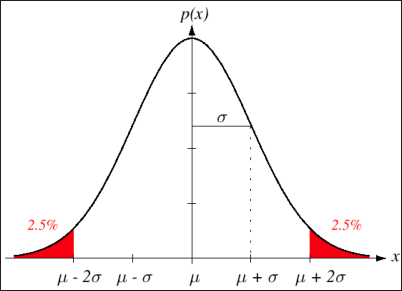
\includegraphics[width=.4\textwidth]{assets/distr-norm-graph.png}
    \caption{Grafico della distribuzione normale}\label{fig:distr-norm-graph}
\end{cimage}
Solo il $5\%$ circa del ``volume'' è esterno all'intervallo $\itc{\mu - 2\si, \mu + 2\si}$.
Solitamente si assume che la distribuzione valga $0$ a distanze maggiori di $3\si$ dal valore medio.
\begin{example}{Stima di $\mu$ e $\si$ per $d = 1$}{}
    Dato un training set di pattern mono-dimensionali composto da $n = 10$ elementi:
    \begin{center}
        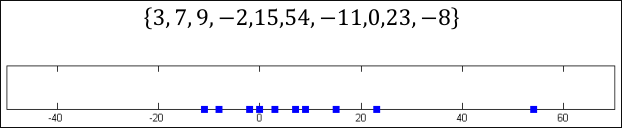
\includegraphics[width=.8\textwidth]{assets/var-med-stima.png}
    \end{center}
    La stima dei parametri per massima verosimiglianza (\textbf{maximum likelihood}) si dimostra essere:
    \begin{itemize}
        \item stima per $\mu$: media campionaria dei valori;
            \[
                \mu = \frac{1}{n}\sum_{i = 1}^n{x_i} = \frac{3 + 7 + 9 + (-2) + 15 + 54 + (-11) + 23 + (-8)}{10} = \frac{90}{10} = 9
            \]
        \item stima per $\si[2]$: varianza campionaria dei valori;
            \[
                \si[2] = \frac{1}{n}\sum_{i = 1}^n{\pt{x_i - \mu}^2} = \cdots = 318.8
            \]
    \end{itemize}
    \begin{center}
        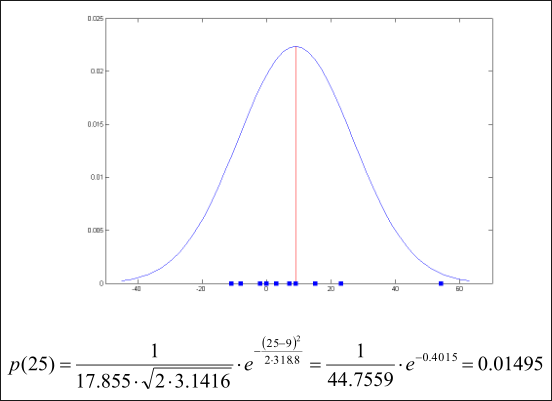
\includegraphics[width=.6\textwidth]{assets/var-med-sol-graph.png}
        \captionof{figure}{Soluzione in forma grafica}\label{fig:var-med-sol-graph}
    \end{center}
    \begin{warning}[Siamo nel continuo]
        $p$ è una densità di probabilità: $\dpb{25}$ non è la probabilità del valore $25$, ma la densità di probabilità nel punto $25$.
        Solo considerando un intervallo di valori, anche piccolo, sulla base possiamo parlare di probabilità.
        In altre parole l'intervallo $\itc{x, x + \id}$ ha probabilità: $\dpb x\id$.
    \end{warning}
\end{example}
% subsection Distribuzione Normale $d=1$ (end)
%
\subsection{Distribuzione Normale Multivariata}\label{sec:distribuzione_normale_multivariata} % (fold)
\begin{note}[Notazione]{}
    Per evitare confusione utilizziamo a pedice l'indice del pattern e (ove necessario) ad apice la componente (scalare):
    \begin{itemize}
        \item $x_i$ pattern i-esimo (vettore);
        \item $x_i^j$ componente j-esima del pattern i-esimo (scalare);
    \end{itemize}
\end{note}
La densità di probabilità nella distribuzione multinormale $d > 1$:
\[
    \dpb{x} = \dfrac{1}{\pt{2\pi}^{d/2}\ab{\Si}^{1/2}} e^{-\dfrac{1}{2}\pt{x - \mu}^t\Si[-1]\pt{x - \mu}}
\]
dove $\mu = \ps{\mu^1, \mu^2, \dots, \mu^d}$ è il \textbf{vettore medio}, e $\Si = \ps{\si[ij]}$ è la \textbf{matrice di covarianza} di dimensione $\pt{d\times d}$.
\emptyln{}
\begin{itemize}
    \item Si assume che i vettori siano di tipo <<colonna>>. L'apice $t$ (trasposto) li trasforma in righe.
    \item $\ab\Si$ e $\Si[-1]$ sono rispettivamente il determinante e l'inversa di $\Si$.
    \item La matrice di covarianza è sempre simmetrica e definita positiva, pertanto ammette l'inversa.
        Essendo simmetrica il numero di parametri che la definisce è $d\cdot \pt{\inc d} / 2$.
    \item Gli elementi diagonali $\si[ii]$ sono le varianze dei rispettivi $x^i$ (ovvero ${\pt{\si[i]}}^2$); gli elementi non diagonali $\si[ij]$ sono le covarianze tra $x^i$ e $x^j$:
        \begin{itemize}
            \item se $x^i$ e $x^j$ sono statisticamente indipendenti, allora $\si[ij] = 0$;
            \item se $x^i$ e $x^j$ sono correlati positivamente, allora $\si[ij] > 0$;
            \item se $x^i$ e $x^j$ sono correlati negativamente, allora $\si[ij] < 0$;
        \end{itemize}
\end{itemize}
%
\paragraph{Rappresentazione Grafica Normale Multivariata}\label{par:rappresentazione_grafica_normale_multivariata} % (fold)
Per $d = 2$ la forma della distribuzione è quella di un'ellisse.
\begin{cimage}
    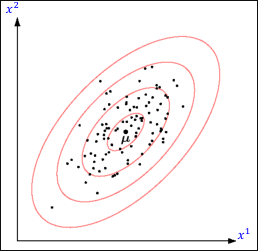
\includegraphics[width=.5\textwidth]{assets/norm-multi-visual.png}
    \caption{Le diverse ellissi individuano luoghi di punti a densità costante}\label{fig:norm-multi-visual}
\end{cimage}
\begin{itemize}
    \item $\mu = \ps{\mu^1, \mu^2}$ controlla la posizione del centro.
    \item $\si[11]$ e $\si[22]$ determinano l'allungamento sui due assi rispetto agli assi cartesiani.
    \item $\si[12] = \si[21]$ controlla la rotazione dell'ellisse rispetto agli assi cartesiani:
        \begin{itemize}
            \item se $= 0$, matrice di covarianza \textit{diagonale}, la distribuzione multinormale è definita come prodotto di $d$ normali monodimensionali. In tal caso gli assi dell'ellisse sono paralleli agli assi cartesiani;
            \item se $> 0$, come in \cref{fig:norm-multi-visual}, $x^1$ e $x^2$ sono positivamente correlate (quando aumenta $x^1$ aumenta anche $x^2$);
            \item se $< 0$, $x^1$ e $x^2$ sono negativamente correlate (quando aumenta $x^1$ cala $x^2$);
        \end{itemize}
    \item gli assi dell'ellisse sono paralleli agli autovalori di $\Si$.
\end{itemize}
% paragraph Rappresentazione Grafica Normale Multivariata (end)
%
\paragraph{Distanza Mahalanobis}\label{par:distanza_mahalanobis} % (fold)
\indent
\begin{definition}{Distanza Mahalanobis}{dist-mahalanobis}
    La \textbf{distanza di Mahalanobis} $r$ tra $x$ e $\mu$, definita dall'equazione:
    \[
        r^2 = \pt{x - \mu}^t\Si[-1]\pt{x - \mu}
    \]
    definisce i bordi a densità costante in una distribuzione multinormale.
\end{definition}
Tale distanza viene spesso utilizzata in sostituzione della distanza euclidea, essendo in grado di ``pesare'' le diverse componenti tenendo conto dei relativi \textbf{spazi di variazione} e della loro \textbf{correlazione}.
\begin{cimage}
    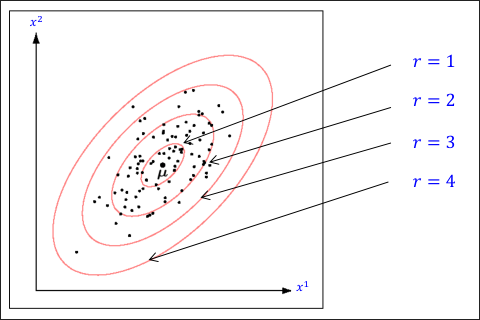
\includegraphics[width=.6\textwidth]{assets/dist-mahalanobis-visual.png}
    \caption{}\label{fig:dist-mahalanobis-visual}
\end{cimage}
Un semplice approccio di <<anomaly detection>> consiste nel fitting gaussiano (calcolo di $\mu$ e $\Si$) dai soli pattern di funzionamento normale del sistema.
I nuovi pattern, la cui distanza di Mahalanobis eccede una soglia data, sono considerati anomalie.
\begin{warning}
    È efficace solo quando la distribuzione dei dati è gaussiana
\end{warning}
% paragraph Distanza Mahalanobis (end)
\paragraph{Esempio stima di $\mu$ e $\si$ con $d = 2$}\label{par:esempio_stima_di_mu_e_si_con_d_} % (fold)
Dato un training set di pattern bi-dimensionali composto da $n = 5$ elementi:
\begin{cimage}
    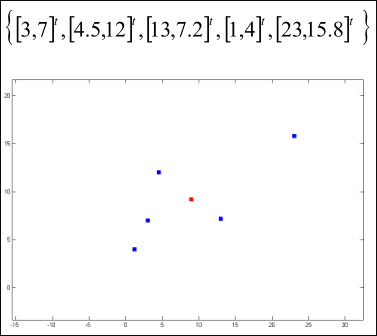
\includegraphics[width=.6\textwidth]{assets/es-stima-mu-si-distr-multi.png}
\end{cimage}
La stima dei parametri per massima verosimiglianza, \textit{maximum likelihood}, è:
\[
    \mu = \begin{bmatrix}
        \mu^1 \\
        \mu^2 \\
        \dots \\
        \mu^d \\
    \end{bmatrix},
    \qquad
    \mu^i = \dfrac{1}{n}\sum_{k = 1,\dots,n}{x+i_k},
    \qquad
    \mu = \begin{bmatrix}
        \frac{3 + 4.5 + 13 + 1 + 23}{5} \\
        \frac{7 + 12 + 7.2 + 4 + 15.8}{5} \\
    \end{bmatrix}
    = \begin{bmatrix}
        8.9 \\ 9.2
    \end{bmatrix}
\]
o in notazione vettoriale:
\[
    \mu = \frac{1}{n}\sum_{i = 1, \dots, n}{x_i}
\]
Successivamente:
\[
    \Si = \begin{bmatrix}
        \si[11] & \si[12] & \cdots & \si[1d] \\
        \si[21] & \si[22] & \cdots & \si[2d] \\
        \cdots & \cdots & \cdots & \dots \\
        \si[d1] & \si[d2] & \cdots & \si[dd] \\
    \end{bmatrix},
    \qquad
    \si[ij] = \frac{1}{n}\sum_{k = 1, \dots, n}{\pt{x_k^i - \mu^i} \cdot \pt{x^j_k - \mu^j}}
\]
o in notazione vettoriale, sia calcolata come somma di matrici ognuna ottenuta come vettore colonna per riga:
\[
    \Si = \dfrac{1}{n}\sum_{i = 1, \dots, n}{\pt{x_i - \mu}\pt{x_i - \mu}^t}
\]
sia come moltiplicazioni tra due matrici dove $X$ è la matrice contenente i pattern nelle colonne, a cui è stata già tolta la media:
\[
    \Si = \dfrac{1}{n}X\T X
\]
\begin{cimage}
    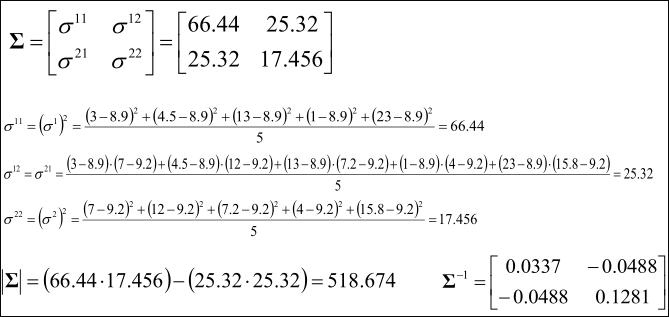
\includegraphics[width=.8\textwidth]{assets/res-es-mu-si-distr-multi.png}
    \caption{Procedimenti conclusivi per ottenere $\Si$}\label{fig:res-es-mu-si-distr-multi}
\end{cimage}
\begin{note}[In forma grafica]{}
    \begin{center}
        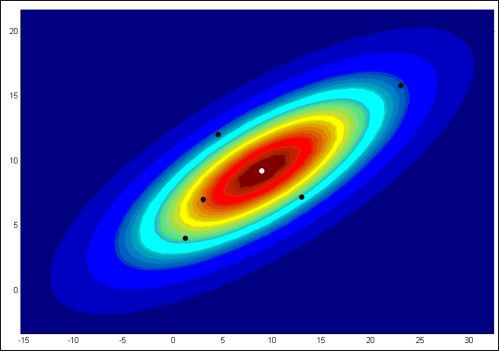
\includegraphics[width=.4\textwidth]{assets/es-mu-si-visual-top.png}
        \captionof{figure}{Vista dall'alto}\label{fig:es-mu-si-visual-top}
    \end{center}
    \begin{center}
        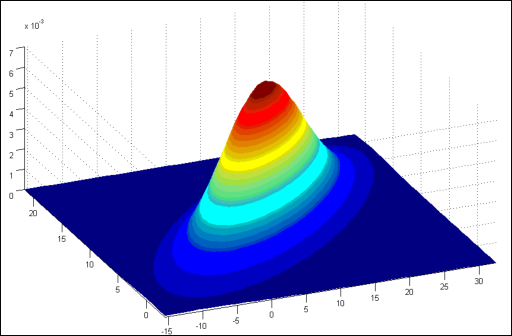
\includegraphics[width=.4\textwidth]{assets/es-mu-si-visual-side.png}
        \captionof{figure}{Vista laterale}\label{fig:es-mu-si-visual-side}
    \end{center}
\end{note}
% paragraph Esempio stima di $\mu$ e $\si$ con $d = 2$ (end)
% subsection Distribuzione Normale Multivariata (end)
%
\subsection{Classificatore di Bayes con distribuzioni Multinormali}\label{sec:classificatore_di_bayes_con_distribuzioni_multinormali} % (fold)
\begin{cimage}
    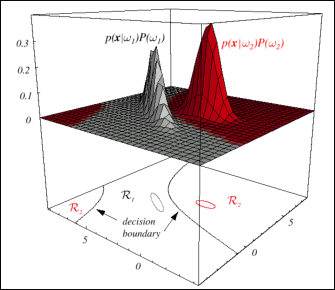
\includegraphics[width=.6\textwidth]{assets/bayes-distri-multi-visual.png}
    \caption{}\label{fig:bayes-distri-multi-visual}
\end{cimage}
In \cref{fig:bayes-distri-multi-visual} sono visualizzate le densità condizionali di $2$ classi di pattern, distribuiti con distribuzione normale $2$-dimensionale, corrette sulla base delle rispettive \textbf{probabilità a priori}.
\\
La classificazione è eseguita utilizzando la regola \textit{Bayesiana}: lo spazio è suddiviso in regioni non connesse, nel caso specifico $\Re_2$ è costituita da due componenti disgiunte.
\begin{definition}{Decision Boundary}{}
    Un \textbf{decision boundary} o \textbf{decision surface} (superficie decisionale) è una zona di confine tra regioni che il classificatore associa a classi diverse; sul boundary la classificazione è ambigua.
    \\
    Le superfici decisionali possono assumere forme diverse, in \cref{fig:bayes-distri-multi-visual} si tratta di due iperboli.
    In generale:
    \begin{itemize}
        \item se le $2$ matrici di covarianza sono \textbf{uguali tra loro}: la superficie decisionale è un \textbf{iper-piano};
        \item se le $2$ matrici di covarianza sono \textbf{arbitrarie}: la superficie decisionale è un \textbf{iper-quadratica};
    \end{itemize}
\end{definition}
% subsection Classificatore di Bayes con distribuzioni Multinormali (end)
%
\subsection{Bayes e confidenza di classificazione}\label{sec:bayes_e_confidenza_di_classificazione} % (fold)
Un grande \textbf{vantaggio} del classificatore di Bayes, rispetto ad altri classificatori, è legato al fatto che esso produce un valore di output probabilistico, scalare compreso fra $0$ e $1$ e con somma pari a $1$ su tutte le classi, che può essere utilizzato come confidenza.
\begin{cimage}
    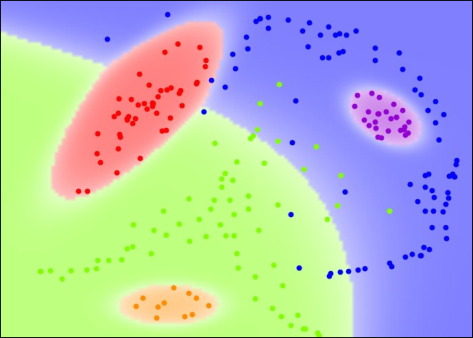
\includegraphics[width=.6\textwidth]{assets/bayes-conf-class.png}
    \caption{Confidenza del classificatore in base al colore}\label{fig:bayes-conf-class}
\end{cimage}
Infatti, un classificatore può assegnare un pattern $x$ a una classe $w_i$ con diversi livelli di certezza (o confidenza) che possono essere impiegati per:
\begin{itemize}
    \item scartare pattern in applicazioni open-set \textbf{con soglia};
    \item costruire un \textbf{multi-classificatore};
\end{itemize}
Se non si è interessati alla confidenza, nella \hyperref[eq:theor-bayes]{formula di Bayes} non è necessario dividere per $\dpb x$ il numeratore, e la regola di Bayes è semplicemente:
\[
    b = \argmax_{i = 1, \dots, s}{\pg{\dba{x}{w_i} \cdot \p{w_i}}}
\]
% subsection Bayes e confidenza di classificazione (end)
\subsection{Bayes parametrico in pratica}\label{sec:bayes_parametrico_in_pratica} % (fold)
Molto spesso si fanno ipotesi azzardate sulla normalità delle densità di probabilità delle classi del problema senza aver sperimentalmente eseguito nessuna verifica; ciò porta a ottenere \textbf{cattivi risultati} di classificazione.
\\
Pertanto, dato un problema con $s$ classi e dato un training set (significativo), deve essere innanzitutto \textbf{valutata la rispondenza alla ``normalità'' delle $s$ distribuzioni}; questo può essere fatto in due modi:
\begin{itemize}
    \item modo \textbf{formale};
    \item modo \textbf{empirico}, visualizzando in vari modi le \textbf{nuvole dei dati} o gli \textbf{istogrammi sulle diverse componenti} e confrontandoli con delle curve teoriche;
\end{itemize}
Una volta provata una normalità delle distribuzioni, si stimano a partire dai dati, vettore medio $\mu$ e matrice di covarianza $\Si$ (maximum likelihood).
\\
Per quanto riguarda le \textbf{probabilità a priori} queste possono essere estratte dalle percentuali di campioni che nel training set appartengono alle diverse classi, o in caso di assenza di informazioni possono essere poste tutte uguali tra loro.
\\
Ogni \textit{nuovo pattern da classificare}, è assegnato a una delle possibili classi in accordo con la regola di Bayes nella quale media e covarianza sono ora note.
\paragraph{Approcci non parametrici e stima delle Densità}\label{par:approcci_non_parametrici_e_stima_delle_densita} % (fold)
Non vengono fatte ipotesi sulle distribuzioni dei pattern e le densità di probabilità sono \textbf{stimate direttamente} dal training set.
\\
Il problema della stima accurata della densità è ritenuto da molti un problema più complesso della classificazione.
\begin{quote}
    In generale la stima delle densità è affrontabile in \textbf{spazi a dimensionalità ridotta} e diventa \textit{critica} al crescere della dimensionalità (\textit{curse of dimensionality}): il volume dello spazio aumenta così tanto che i pattern diventano troppo sparsi.
\end{quote}
\begin{critical}
    In uno spazio dove i pattern sono molto sparsi occorrono molti più esempi per fare stime di dimensionalità affidabili.
    \\
    La \textbf{riduzione di dimensionalità} è una delle tecniche possibili per contrastare la \textbf{curse of dimensionality}.
\end{critical}
% paragraph Approcci non parametrici e stima delle Densita (end)
% subsection Bayes parametrico in pratica (end)
%
\subsection{Stima della Densità}\label{sec:stima_della_densita} % (fold)
La probabilità che un pattern $x$ cada all'interno di $\Re$ è:
\[
    P_1 = \int_{\Re}{\dpb{x'}\,\id[x']}
\]
Dati $n$ pattern indipendenti, la probabilità che $k$ di questi cadano nella regione $\Re$ è calcolabile attraverso la \textbf{distribuzione binomiale}:
\[
    P_k = \binom{n}{k}P_1^k\pt{1 - P_1}^{n-k}
\]
il cui valore medio è $k = n \cdot P_1$, e quindi $P_1 = k / n$.
\emptyln{}
Assumendo che la regione $\Re$, di volume $V$, sia piccola e che quindi $\dpb{\cdot}$ non vari significativamente all'interno di essa:
\[
    P_k = \int_{\Re}\dpb{x'}\,\id[x'] \approx \dpb x \cdot V
\]
\begin{equation}\label{eq:stima-dens}
    \dpb{x} = \dfrac{P_1}{V} = \dfrac{k}{n \cdot V}
\end{equation}
%
% subsection Stima della Densita (end)
%
\subsection{Parzen Window}\label{sec:parzen_window} % (fold)
La regione $\Re$, denominata finestra (\textbf{Window}), è costituita da un ipercubo $d$-dimensionale, definito dalla funzione $\vphi$:
\[
    \fvphi{u} = \begin{cases}
        1 & \ab{u_j} \le \dhalf,\, j = 1, \dots, d \\
        0 & \text{altrimenti}
    \end{cases}
\]
Dato un generico ipercubo centrato in $x$ e avente lato $h_n$ (e quindi volume $V_n = h_n^d$) il numero di pattern del training set che cadono all'interno dell'iper-cubo è dato da:
\[
    k_n = \sum_{i = 1}^n{\fvphi{\frac{x_i - x}{h_n}}}
\]
sostituendo $k_n$ a \cref{eq:stima-dens} si ottiene:
\[
    p_n\pt x = \dfrac{1}{n\cdot V_n}\sum_{i = 1}^n{\fvphi{\frac{x_i - x}{h_n}}},
    \qquad
    \text{dove } V_n = h_n^d
\]
Ovviamente, specie nel caso in cui il numero di pattern non sia elevato, la \red{dimensione} della finestra $V_n$, e quindi il lato $h_n$, ha un \red{forte impatto} sul risultato, infatti:
\begin{itemize}
    \item se la finestra è \textbf{piccola}, la stima risulta piuttosto ``rumorosa'', molto attratta dai campioni e statisticamente instabile;
    \item se la finestra è \textbf{grande}, la stima è più stabile ma piuttosto vaga e sfocata;
\end{itemize}
Si dimostra che per ottenere \hyperref[sub:convergenza]{convergenza}, la dimensione della finestra deve essere calcolata tenendo conto del numero di campioni del training set:
\[
    V_n = \frac{V_1}{\sqrt{n}},
    \qquad
    \text{dove }\ V_1 \text{ (o \red{$h_1$}) è un \red{iperparametro}}
\]
%
\paragraph{Parzen Window con Soft Kernel}\label{par:parzen_window_con_soft_kernel} % (fold)
Nella pratica, invece di funzioni finestra ipercubo si utilizzano \textbf{kernel function} più \textbf{soft} grazie alle quali ogni pattern $x_i$ contribuisce alle stime di densità in un intorno di $x$ in accordo con la distanza da $x$.
In questo modo le \red{superfici decisionali} risultano molto più regolari (\red{smoothed}).
\begin{definition}{Kernel Function}{}
    Le \textbf{kernel function} devono essere funzioni densità (sempre $\ge 0$ e con integrale su tutto lo spazio uguale a $1$).
    Utilizzando la funzione \hyperref[sec:distribuzione_normale_multivariata]{multinormale} (con $\mu = \ps{0, \dots, 0}$ e $\Si = I$):
    \[
        \fvphi{u} = \dfrac{1}{\pt{2\pi}^{d/2}} e^{-\dfrac{u^t u}{2}}
    \]
\end{definition}
\begin{cimage}
    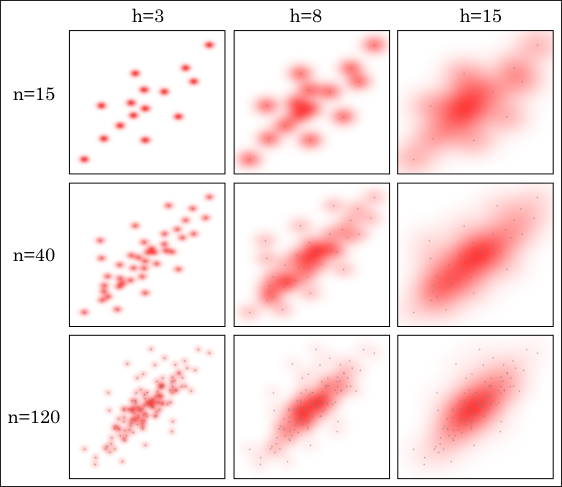
\includegraphics[width=.8\textwidth]{assets/parzen-soft-kern.png}
\end{cimage}
% paragraph Parzen Window con Soft Kernel (end)
% subsection Parzen Window (end)
% section Classificatore di Bayes (end)
%
\section{Nearest Neighbor}\label{sec:nn} % (fold)
Data una metrica $dist\pt\cdot$ nello spazio multidimensionale, il classificatore \textbf{nearest neighbor}, classifica un pattern $x$ con la stessa classe dell'elemento $x'$ a esso più vicino nel training set \red{TS}:
\[
    \dist{x}{x'} = \min_{x_i \in TS}{\pg{\dist{x}{x_i}}}
\]
\begin{quote}
    Invece di derivare dai dati le distribuzioni condizionali delle classi per poi far uso della \hyperref[sub:classificatore_di_bayes]{regola di Bayes} per la classificazione, questo classificatore cerca in modo \red{piuttosto pragmatico} di massimizzare direttamente la probabilità a posteriore; infatti se $x'$ è molto vicino a $x$ è lecito supporre che:
    \[
        \ba{w_i}{x} \approx \ba{w_i}{x}
    \]
    In effetti si può dimostrare che la probabilità di errore $P$ della regola nearest neighbor \red{non è mai peggiore del doppio del minimo errore possibile} $P^*$ (quello Bayesiano).
    \begin{center}
        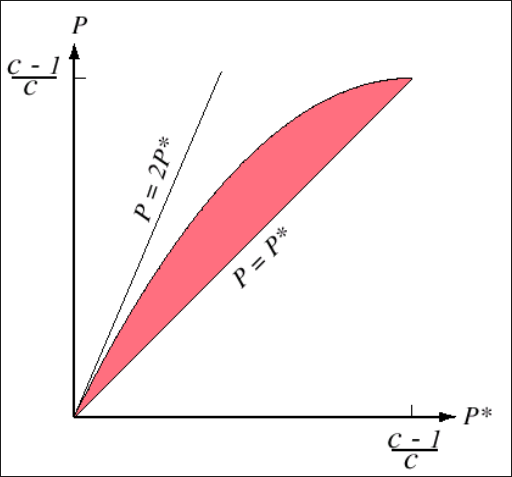
\includegraphics[width=.3\textwidth]{assets/err-nn-bayes-visual.png}
    \end{center}
    Nella pratica, questo non significa però che l'approccio Bayesiano fornisca sempre risultati migliori di nearest neighbor, infatti se la stima delle densità condizionali è poco accurata i risultati del classificatore Bayesiano possono essere peggiori.
\end{quote}
\begin{example}{Esempio NN}{}
    Nell'esempio visto in precedenza, \cref{ex:maschi-femmine-bayes}, la regola \textit{NN} assegna il pattern $x$ alla classe $w_1$ (maschi --- blu).
    La \cref{fig:nn-5-classi-visual} mostra il partizionamento dello spazio operato dalla regola NN su un training set con $5$ classi:
    \begin{center}
        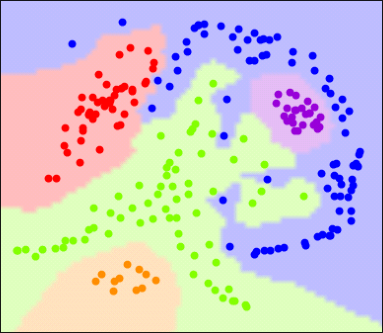
\includegraphics[width=.4\textwidth]{assets/nn-5-classi-visual.png}
        \captionof{figure}{}\label{fig:nn-5-classi-visual}
    \end{center}
\end{example}
    %
\subsection{k-NN}\label{sec:k_nn} % (fold)
La regola \hyperref[sec:nn]{nearest neighbor} produce un partizionamento dello spazio, noto come \red{tassellazione di Voronoi}:
\begin{cimage}
    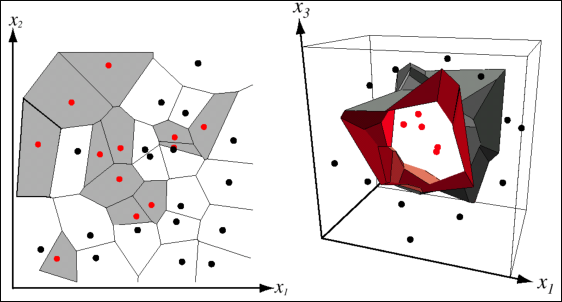
\includegraphics[width=.6\textwidth]{assets/tass-voronoi-visual.png}
    \caption{Rappresentazione grafica della tassellazione di Voronoi}\label{fig:tass-voronoi-visual}
\end{cimage}
Ogni elemento $x_i \in TS$ determina un tassello, all'interno del qualie i pattern saranno assegnati alla stessa classe di $x_i$.
\\
La regola di classificazione nearest neighbor è piuttosto radicale; infatti basta che un elemento del training set non sia molto ``affidabile'' (\red{outlier}) affinché tutti i pattern nelle sue vicinanze siano in seguito etichettati non correttamente.
\begin{quote}
    Un modo generalmente più robusto, che può essere visto come estensione della regola nearest neighbor è il cosiddetto classificatore \red{k-nearest neighbor}.
\end{quote}
\begin{definition}{$k$-nn}{knn}
    La regola \red{$k$-Nearest Neighbor} ($k$-nn) determina i $k$ elementi più vicini al pattern $x$ da classificare ($k$ è un \textbf{\hyperref[def:iperparam]{iperparametro}}); ogni pattern tra i $k$ vicini vota per la classe cui esso stesso appartiene; il pattern $x$ viene assegnato alla classe che ha ottenuto il maggior numero di voti.
\end{definition}
\begin{cimage}
    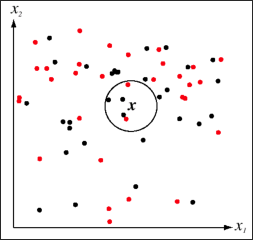
\includegraphics[width=.4\textwidth]{assets/knn-es.png}
    \caption{Il classificatore $5$-NN assegna $x$ alla classe ``nera'' in quanto ha ricevuto $3$ voti su $5$}\label{fig:knn-es}
\end{cimage}
\begin{warning}
    Nel caso di $2$ classi è bene scegliere $k$ dispari per evitare pareggi indesiderati.
\end{warning}
Per $TS$ infiniti la regola di classificazione $k$-NN si dimostra migliore di $1$-NN (\hyperref[sub:nn]{NN}), e all'aumentare di $k$, l'errore $P$ converge all'errore Bayesiano.
\begin{cimage}
    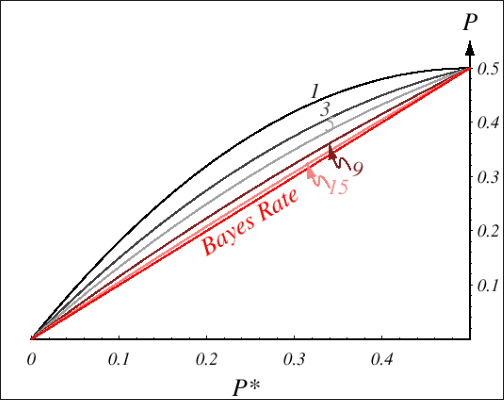
\includegraphics[width=.4\textwidth]{assets/err-knn-bayes-visual.png}
    % \caption{}\label{fig:err-knn-bayes-visual}
\end{cimage}
Nella pratica ($TS$ limitati), \textbf{aumentare $k$} significa estendere l'ipersfera di ricerca andando a sondare la probabilità a posteriori \red{lontano dal punto di interesse}; il valore ottimale di $k$ (\red{solitamente $< 10$}) deve essere determinato su un validation set separato.
\begin{example}{Esempio $k$-NN}{}
    \begin{center}
        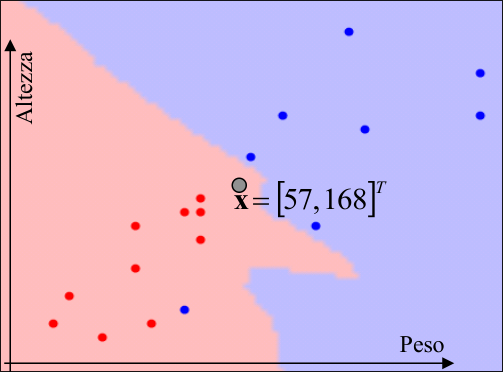
\includegraphics[width=.4\textwidth]{assets/es-mf-knn-visual.png}
    \end{center}
    Nell'esempio visto in precedenza, \cref{ex:maschi-femmine-bayes}, la regola \textit{$k$-NN} assegna il pattern $x$ alla classe $w_2$ (femmine --- rossi).
    \emptyln{}
    L'animazione successiva mostra il partizionamento dello spazio operato dalla regola $k$-NN sul training set con $5$ classi visto in precedenza al variare di $k$.
    \begin{center}
        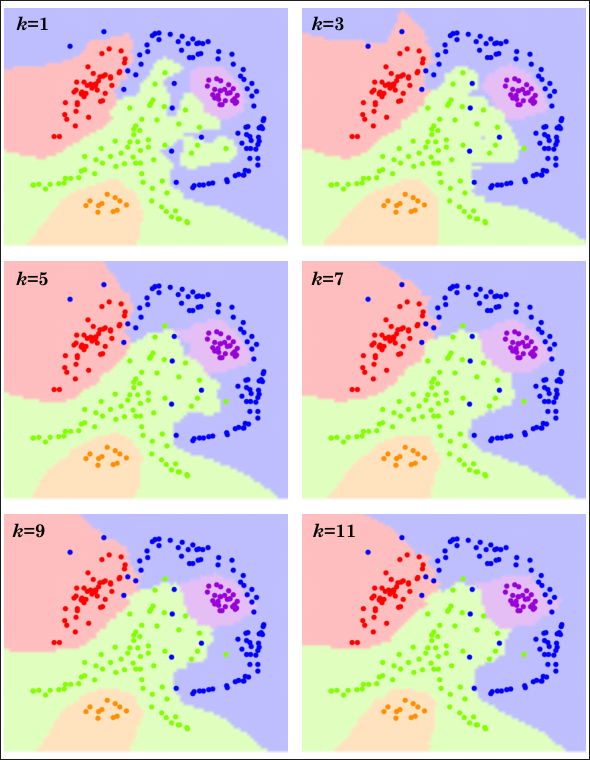
\includegraphics[width=.7\textwidth]{assets/anim-knn-visual.png}
        \captionof{figure}{Variazione di $k = 1,3,5,7,9,11$}\label{fig:anim-knn-visual}
    \end{center}
\end{example}
\paragraph{Confidenza di Classificazione}\label{par:confidenza_di_classificazione} % (fold)
Da un classificatore $k$-NN risulta piuttosto semplice estrarre una \textbf{confidenza} (probabilistica) circa la classificazione eseguita; siano:
\[
    \ps{v_1, v_2, \dots, v_s},
    \qquad
    \sum_{i = 1}^s{v_i} = k
\]
i voti ottenuti dal pattern $x$, allora le \red{confidenze} (sfumature in \cref{fig:knn-conf-visual}) possono essere semplicemente ottenute dividendo per $k$ i voti ottenuti:
\[
    \ps{\frac{v_1}{k}, \frac{v_1}{k}, \ldots, \frac{v_s}{k}}
\]
\begin{cimage}
    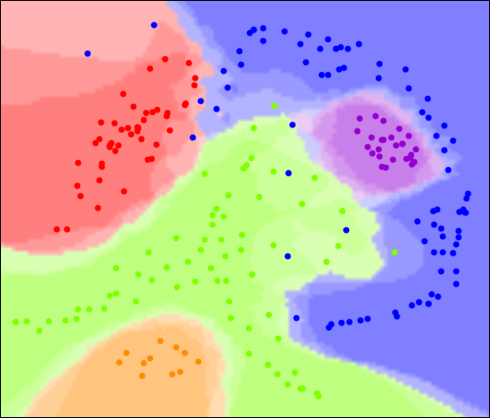
\includegraphics[width=.4\textwidth]{assets/knn-conf-visual.png}
    \caption{}\label{fig:knn-conf-visual}
\end{cimage}
% paragraph Confidenza di Classificazione (end)
%
\paragraph{Complessità Computazionale}\label{par:complessita_computazionale} % (fold)
L'utilizzo di un classificatore NN o $k$-NN nel caso di training set di elevate dimensioni può diventare problematico:
\begin{itemize}
    \item è necessario \red{memorizzare} tutti i pattern del \hyperref[def:ts]{Training Set};
    \item per ogni classificazione è necessario \red{calcolare la distanza} del pattern da classificare da tutti i pattern del training set e ordinare parzialmente le distanze per ottenere quelle più piccole;
\end{itemize}
\begin{warning}
    Tecniche di \textit{editing/condensing} possono alleviare questo problema, ma quando l'efficienza è importante è sconsigliabile indicizzare i dati attraverso strutture spaziali (es. \red{kd-tree}) che consentono di individuare i vicini senza effettuare una scansione esaustiva.
\end{warning}
% paragraph Complessita Computazionale (end)
%
\paragraph{Prototipi di Classi}\label{par:prototipi_di_classi} % (fold)
Talvolta nella classificazione nearest neighbor invece di mantenere tutti i pattern del $TS$ e calcolare la distanza da ciascuno di essi, si preferisce \red{selezionare/derivare} da essi uno o più \textbf{prototipi} per ciascuna classe e utilizzare questi ultimi per la classificazione come se fossero i soli elementi di $TS$.
Queste tecniche prendono il nome di:
\begin{itemize}
    \item \textbf{editing}: quando si cancellano solo pattern dal training set, senza derivare nuovi pattern;
    \item \textbf{condensing}: se i prototipi non appartenevano al $TS$ e sono stati derivati;
\end{itemize}
\begin{cimage}
    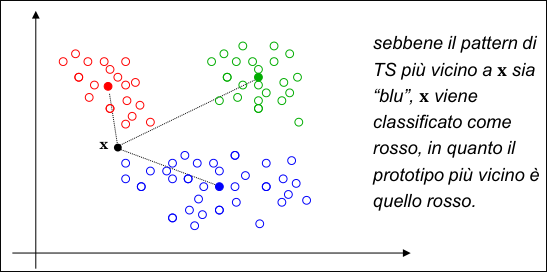
\includegraphics[width=.8\textwidth]{assets/nn-prot-edit-conds.png}
    \caption{}\label{fig:nn-prot-edit-conds}
\end{cimage}
Ciò comporta i seguenti \textbf{vantaggi}:
\begin{itemize}
    \item non è necessario calcolare un elevato numero di distanze;
    \item i prototipi sono spesso più affidabili e robusti di singoli pattern;
\end{itemize}
Un singolo prototipo di classe può essere \red{derivato} come vettore medio dei vettori di quella classe nel $TS$.
Processi di \textit{vector quantization} o clustering consentono di ottenere più prototipi per ogni classe.
% paragraph Prototipi di Classi (end)
% subsection k-NN (end)
%
\subsection{NN e Metriche}\label{sec:metriche} % (fold)
Il comportamento della regola $k$-NN è strettamente legato alla metrica (funzione distanza) adottata.
La \red{distanza euclidea}, che rappresenta il caso $L_2$ nella definizione di metriche di Minkowsky, è sicuramente la metrica più utilizzata.
\begin{equation}\label{eq:dis_euclidea}
    L_k\pt{a,\,b} = \pt{\sum_{i = 1}^d {\ab{a_i - b_i}^k}}^{1/k}
\end{equation}
Nella pratica, prima di adottare semplicemente la dispanza euclidea è bene valuratre lo spazio di variazione delle componenti (o \red{feature}) e la presenza di eventuali forti correlazioni tra le stesse.
\\
Supponiamo ad esempio di voler classificare le persone sulla base dell'altezza e della lunghezza del piede.
Ogni pattern $x$ (bidimensionale) risulta costituito da due feature: $x_1 =$ altezza, $x_2 =$ lunghezza del piede.
\begin{cimage}
    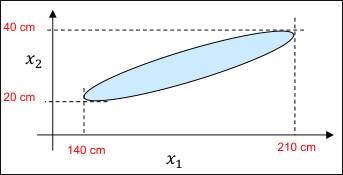
\includegraphics[width=.4\textwidth]{assets/es-met-visual.png}
\end{cimage}
Lo \red{spazio di variazione} dell'altezza ($210-140$) risulta maggiore di quello della lunghezza del piede ($40 - 20$).
Pertanto se la similarità tra pattern venisse misurata con semplice distanza euclidea la componente altezza ``peserebbe'' di più della componente lunghezza del piede.
%
\paragraph{Normalizzazione}\label{par:normalizzazione} % (fold)
Per evitare i problemi legati ai diversi spazi di variazioni delle feature, particolarmente fastidiosi per alcune tecniche, è consigliato di normalizzare i pattern.
Le \textbf{normalizzazioni} più comuni sono: \textbf{min-max scaling} e \textbf{standardization}.
\begin{definition}{Min-Max Scaling}{}
    Per ogni feature $i$-esima si calcolano il massimo $\max_i$ e il minimo $\min_i$ e si applica una trasformazione lineare (scaling) che <<tipicamente>> mappa $\min_i$ a $0$ e $\max_i$ a $1$.
    \[
        x' = \frac{\pt{x - \min_i}}{\pt{\max_i - \min_i}}
    \]
\end{definition}
\begin{definition}{Standardization}{}
    Per ogni feature $i$-esima si calcola la media $mean_i$ e la deviazione standard $stddev_i$ e si trasformano i valori come:
    \[
        x' = \frac{x - mean_i}{stddev_i}
    \]
    Dopo la trasformazione tutte le feature hanno, sul training set, media $0$ e deviazione standard $1$.
\end{definition}
\begin{critical}
    I parametri della normalizzazione, come minimo e massimo, si calcolano \textbf{\red{sul solo training set}} e la trasformazione si applica a tutti i dati (training, validation, test).
    Nel caso di \red{$k$-fold cross-validation} la normalizzazione dovrebbe essere ripetuta $k$ volte (uso di \textit{pipeline} in scikit-learn).
\end{critical}
Le semplici tecniche sopra descritte operano sulle singole feature indipendentemente.
Una tecnica di normalizzazione efficace, ma più costosa, che opera simultaneamente su tutte le feature, tenendo conto della loro correlazione, è la \textbf{\red{Whitening transform}} (o PCA whitening).
Molto in voga prima del deep-learning, ormai poco utilizzata.
% paragraph Normalizzazione (end)
\paragraph{Whitening Transform}\label{par:whitening_transform} % (fold)
Un'efficace normalizzazione rispetto agli spazi di variazione, in grado anche di tener conto delle correlazioni tra feature è possibile:
\begin{itemize}
    \item pre-normalizzando lo spazio delle feature attraverso Whitening transform;
    \item utilizzando come metrica la \hyperref[def:dist-mahalanobis]{distanza di Mahalanobis};
\end{itemize}
Le due alternative sono \red{equivalenti}.
Nel primo caso l'ellissoide corrisponde allo spazio delle feature viene ``sfericizzato'' a priori e viene in seguito usata la distanza euclidea; nel secondo la distanza di Mahalanobis normalizza ogni componente sulla base della matrice di covarianza $\Si$.
\begin{cimage}
    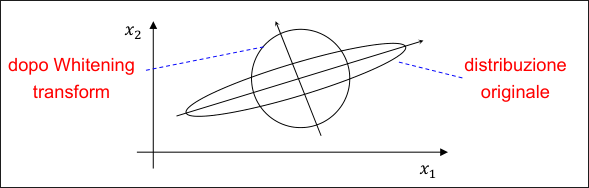
\includegraphics[width=.8\textwidth]{assets/2-norm-effect-visual.png}
    \caption{}\label{fig:2-norm-effect-visual}
\end{cimage}
\begin{note}
    Da non sottovalutare l'importanza della correlazione tra features come \red{aspetto negativo per la classificazione}.
    Infatti, l'utilizzo di feature correlate \textbf{riduce} (anche drasticamente) il potere discriminante.
    Nel caso ideale \red{tutte le feature sono statisticamente indipendenti}.
    \emptyln{}
    Due feature altamente discriminanti se prese individualmente, ma tra loro fortemente correlate, sono nel complesso meno discriminanti di una terza feature leggermente più discriminante di ognuna delle precedenti.
\end{note}
La distanza di Mahalanobis, o la sfericizzazione dello spazio, \textbf{tiene conto delle correlazioni} e pesa maggiormente feature non correlate.
% paragraph Whitening Transform (end)
\paragraph{Metric Learning}\label{par} % (fold)
Un approccio più generale alla scelta della metrica da utilizzare in una determinata applicazione, consiste nel learning \red{supervisionato} della metrica stessa dai dati del training set.
L'obiettivo è quello di determinare una trasformazione degli input che:
\begin{itemize}
    \item <<avvicini>> pattern della stessa classe;
    \item <<allontani>> pattern di classi diverse;
\end{itemize}
La distanza euclidea nello spazio originale è pari a:
\[
    \dist{a}{b} = \sqrt{\pt{a-b}^t \pt{a-b}} = \nm{a-b}_2
\]
Un tipico approccio di metric learning lineare determina, con un training supervisionato, una matrice $G$ che trasforma gli input, e continua ad applicare la distanza euclidea agli input trasformati:
\[
    \dist{a}{b} = \nm{Ga - Gb}_2
\]
Sono possibili anche approcci \red{non lineari}:
\[
    \dist{a}{b} = \nm{G\fphi a - G\fphi b}_2
\]
dove $\phi$ è una funzione \red{non lineare}.
% paragraph Metric Learning (end)
\paragraph{Similarità e Distanza Coseno}\label{par:similarita_e_distanza_coseno} % (fold)
Una similarità/distanza piuttosto utilizzata in applicazioni di \textit{information retrieval}, \textit{data mining} e \textit{text mining} è la \textbf{similarità coseno}.
\begin{definition}{Similarità Coseno}{sim-cos}
    Geometricamente, dati due vettori $a$ e $b$ la \textbf{similarità coseno} corrisponde al coseno dell'angolo tra di essi:
    \[
        \cssm{a}{b} = \dfrac{a^t \cdot b}{\nm a \cdot \nm b}
    \]
    è noto infatti che il prodotto scalare tra due vettori è:
    \[
        a^t \cdot b = \nm a \cdot \nm b \cdot \cos{\pt{\te}}
    \]
    Due vettori identici hanno similarità $1$ e due vettori opposti $-1$.
\end{definition}
\begin{definition}{Distanza Coseno}{dis-cos}
    La \textbf{distanza coseno} è semplicemente:
    \[
        \csds{a}{b} = 1 - \cssm{a}{b}
    \]
\end{definition}
\begin{example}{Esempio di un Confronto di Testi}{}
    Un testo può essere codificato da un vettore numerico dove ogni dimensione contiene il numero di occorrenze di una certa parola rispetto a un dato dizionario.
    La similarità di contenuto tra due testi non dipende dal numero assoluto di parole ma dalla frequenza relativa di ciascuna di esse.
    \red{La distanza coseno <<sconta>> la lunghezza dei due vettori}.
\end{example}
\begin{note}
    La distanza coseno non è una metrica, ad esempio non rispetta la diseguaglianza triangolare.
    Se si è interessati a una metrica si può passare alla \textbf{distanza angolare}.
\end{note}
\begin{definition}{Distanza Angolare}{dis-ang}
    \[
        \ands{a}{b} = \dfrac{\inv\cos{\pt{\cssm{a}{b}}}}{\pi}
    \]
\end{definition}
% paragraph Similarita e Distanza Coseno (end)
% subsection Metriche (end)
% section Nearest Neighbor (end)
%
\section{SVM}\label{sub:svm} % (fold)
La \red{teoria} che governa i meccanismi di funzionamento di \ac{svm} è stato introdotta da \textbf{Vapnik} a partire dal 1965 e perfezionata recentemente.
\ac{svm} è uno degli strumenti più utilizzati per la classificazione dei pattern.
\\
Invece di stimare la densità di probabilità delle classi, Vapnik suggerisce di risolvere direttamente il problema di interesse, ovvero \textbf{determinare le superfici decisionali tra le classi} \red{classification boundaries}.
\begin{itemize}
    \item \ac{svm} \textbf{lineare} (la superficie di separazione è un \red{iperpiano}) e pattern del training set \textbf{linearmente separabili};
    \item \ac{svm} \textbf{lineare} e pattern \textbf{non linearmente separabili}. Ci saranno inevitabilmente errori di classificazione nel training set non esistendo alcun iperpiano in grado di separare i pattern;
    \item \ac{svm} \textbf{non lineare} senza ipotesi sulla separabilità;
    \item estensione \textbf{multiclasse};
\end{itemize}
\subsection{Idea alla Base}\label{sub:idea_alla_base} % (fold)
Date due classi di pattern multidimensionali linearmente separabili, tra tutti i possibili iperpiani di separazione, \ac{svm} determina quello in grado di \red{separare le classi} con maggiore \textbf{margine} possibile.
\begin{quote}
    Il \textbf{margine} è la distanza minima di punti delle due classi nel training set dall'iperpiano idividuato.
\end{quote}
\begin{cimage}
    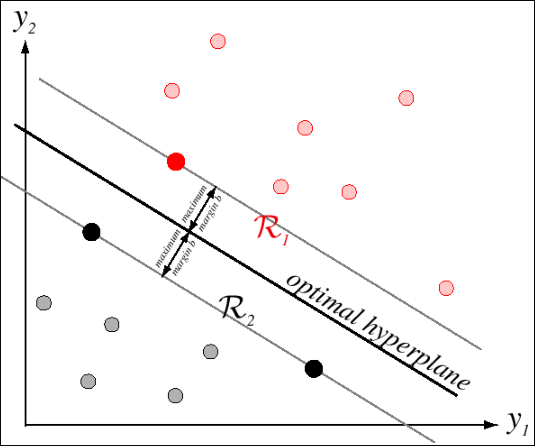
\includegraphics[width=.4\textwidth]{assets/svm-idea-visual.png}
\end{cimage}
La massimizzazione del margine è legata alla \textbf{generalizzazione}.
Se i pattern del training set sono classificati con ampio margine si può <<sperare>> che anche i pattern del test set vicini al confine tra le classi siano gestiti correttamente.
% subsection Idea alla Base (end)
%
\subsection{SVM Lineari}\label{sub:svm_lineari} % (fold)
\subsubsection{Pattern Separabili}\label{sec:pattern_separabili} % (fold)
Date due classi di pattern (\textbf{linearmente separabili}), e un training set $TS$ contenente $n$ campioni $\pt{x_1, y_1},\, \dots, \pt{x_n, y_n}$, dove $x_i \in \Re^d$ sono i \red{pattern multidimensionali} e $y_i \in \pg{+1,\, -1}$ le \red{etichette} delle due classi, esistono diversi iperpiani in grado di eseguire la separazione voluta.
\begin{definition}{Iperpiano}{}
    Un generico iperpiano è definito dai parametri $\pt{w,\,b}$:
    \[
        D\pt x = w \cdot x + b
    \]
    dove:
    \begin{itemize}
        \item $w$ è il vettore normale all'iperpiano;
        \item $b / \nm w$ è la distanza dall'origine;
        \item $D\pt x = 0$ è il luogo dei vettori sul piano;
        \item \[
                x = x_p + r\dfrac{w}{\nm w},
                \qquad
                D\pt x_p = 0
            \]
    \end{itemize}
    \begin{center}
        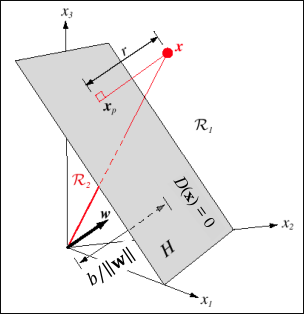
\includegraphics[width=.4\textwidth]{assets/linear-iperpiano-def.png}
    \end{center}
    \[
        D\pt x = w \cdot x + b = r \cdot \nm w
    \]
    La \textbf{distanza} di un vettore $x$ dall'iperpiano vale pertanto:
    \[
        r = \dfrac{D \pt x}{\nm w}
    \]
    Gli iperpiani $\pt{w,\,b}$ che separano i pattern del $TS$, con distanza minima $1 / \nm w$ su ogni lato, soddisfano, per $i = 1,\,\dots,\,n$, le equazioni:
    \[
        \begin{matrix}
            w \cdot x_i + b \ge +1 \qquad \text{se } y_i = +1 \\
            w \cdot x_i + b \le -1 \qquad \text{se } y_i = -1
        \end{matrix}
    \]
    o in modo più compatto:
    \[
        y_i\ps{w \cdot x_i + b} \ge 1 \qquad \text{per } i = 1,\,\dots,\,n
    \]
\end{definition}
\begin{definition}{SVM Margine}{}
    La \red{minima distanza} tra l'iperpiano di separazione e un pattern del training set è detta \textbf{margine} ($\tau$).
    \begin{center}
        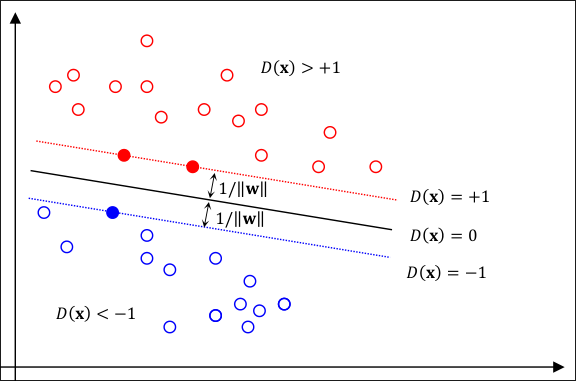
\includegraphics[width=.4\textwidth]{assets/margine-def-es.png}
        \captionof{figure}{Margine tra l'iperpiano e un pattern del $TS$}\label{fig:margine-def-es}
    \end{center}
    La distanza dei punti che giacciono sull'iperpiano $D\pt x = +1$ dall'iperpiano di separazione è $1 / \nm w$; lo stesso vale per i punti sull'iperpiano $D\pt x = -1$.
    \\
    Pertanto il \red{margine} è $\tau = \dfrac{2}{\nm w}$.
\end{definition}
L'iperpiano \textbf{ottimo} secondo \ac{svm} è quello che soddisfa i vincoli di separazione dei pattern e \textbf{massimizza il margine $\tau$}.
\[
    \begin{aligned}
        \text{Minimizza:}&\qquad \nm w ^2 / 2 \\
        \text{Vincoli:}&\qquad y_i\ps{w \cdot x_i + b} \ge 1 \qquad \text{per } i = 1,\,\dots,\,n
    \end{aligned}
\]
I pattern del training set che giacciono sul margine (cerchi pieni in \cref{fig:margine-def-es}) sono detti \textbf{support vector}.
Tali pattern, che costituiscono i casi più complessi, definiscono completamente la soluzione del problema, che può essere espressa come \red{funzione di solo tali pattern}, indipendentemente dalla dimensionalità dello spazio $d$ e dal numero $n$ di elementi in $TS$.
% subsubsection Pattern Separabili (end)
% subsection SVM Lineari (end)
%
\subsection{Lineari: pattern linearmente separabili e non}\label{sec:lineari_pattern_linearmente_separabili_e_non} % (fold)

% subsection Lineari: pattern linearmente separabili e non (end)
%
\subsection{Non lineari}\label{sec:non_lineari} % (fold)

% subsection Non lineari (end)
%
\subsection{Caso multiclasse}\label{sec:caso_multiclasse} % (fold)

% subsection Caso multiclasse (end)
% section SVM (end)
%
\section{Multi classificatori}\label{sub:multi_classificatori} % (fold)
%
\subsection{Fusione a livello di decisione}\label{sec:fusione_a_livello_di_decisione} % (fold)

% subsection Fusione a livello di decisione (end)
%
\subsection{Fusione a livello di confidenza}\label{sec:fusione_a_livello_di_confidenza} % (fold)

% subsection Fusione a livello di confidenza (end)
%
\subsection{Random Forest (Bagging)}\label{sec:random_forest_bagging_} % (fold)

% subsection Random Forest (Bagging) (end)
%
\subsection{AdaBoost (Boosting)}\label{sec:adaboost_boosting_} % (fold)

% subsection AdaBoost (Boosting) (end)
%
\subsection{Gradient Boosting}\label{sec:gradient_boosting} % (fold)

% subsection Gradient Boosting (end)
% section Multi classificatori (end)
% chapter Classificazione (end)

